% Лабораторная работа по АСиСу № 5
% Михедов Константин Константинович

% Тип документа: статья, на бумаге А4
\documentclass[a4paper]{article}

% Подключение сторонних tex файлов 
\usepackage{import}


% Основные данные - ВУЗ, факультет, город...
\import{./../../stuff/tex}{config.tex}

% Подключение необходимых зависимостей
\import{./../../stuff/tex/settings}{packages.tex}
% Настройка подключенных пакетов
\import{./../../stuff/tex/settings}{preferences.tex}


% Шаблон титульной страницы 
\import{./../../stuff/tex/templates}{title.tex}
% Упрощенный блок "выполнил"
\import{./../../stuff/tex/templates}{sign1.tex}
% Макрос для содержания
\import{./../../stuff/tex/templates}{toc.tex}

% Определяем название документа
\title{
  Лабораторная работа №5 по курсу \\
  <<Компьютерный практикум <<Администрирование систем и сетей>>  
}
% Отключаем отображение правительства
\renewcommand{\government}{}
% Отключаем сокращенное нзавание университета
\renewcommand{\subuniversity}{}
% Указываем преподавателя
\renewcommand{\shortteachername}{Зудин Д.Е.}


% Путь до внешних изображений
\graphicspath{ {./figures/}}


% Основной текст работы
\begin{document}
  \templatedtitlepage
  
  \toc
  \section{Ход работы}

  \subsection{Общий анализ}

  Для начала проверим доступность следующих ресурсов: \href{lacninc.net}{lacnic.net} (месторасположение - Южная Америка),
  \href{apnic.net}{apnic.net} (месторасположение - Австралия), \href{afrinic.net}{afrinit.net} (месторасположение - Африка) и \href{yandex.ru}{yandex.ru} (месторасположение - Российская Федерация).
  Чтобы сделать это - воспользуемся встроенной утилитой \textit{ping} (рис. \ref{img:0001} на стр. \pageref{img:0001}):
  \begin{figure}[H]
    \centering
    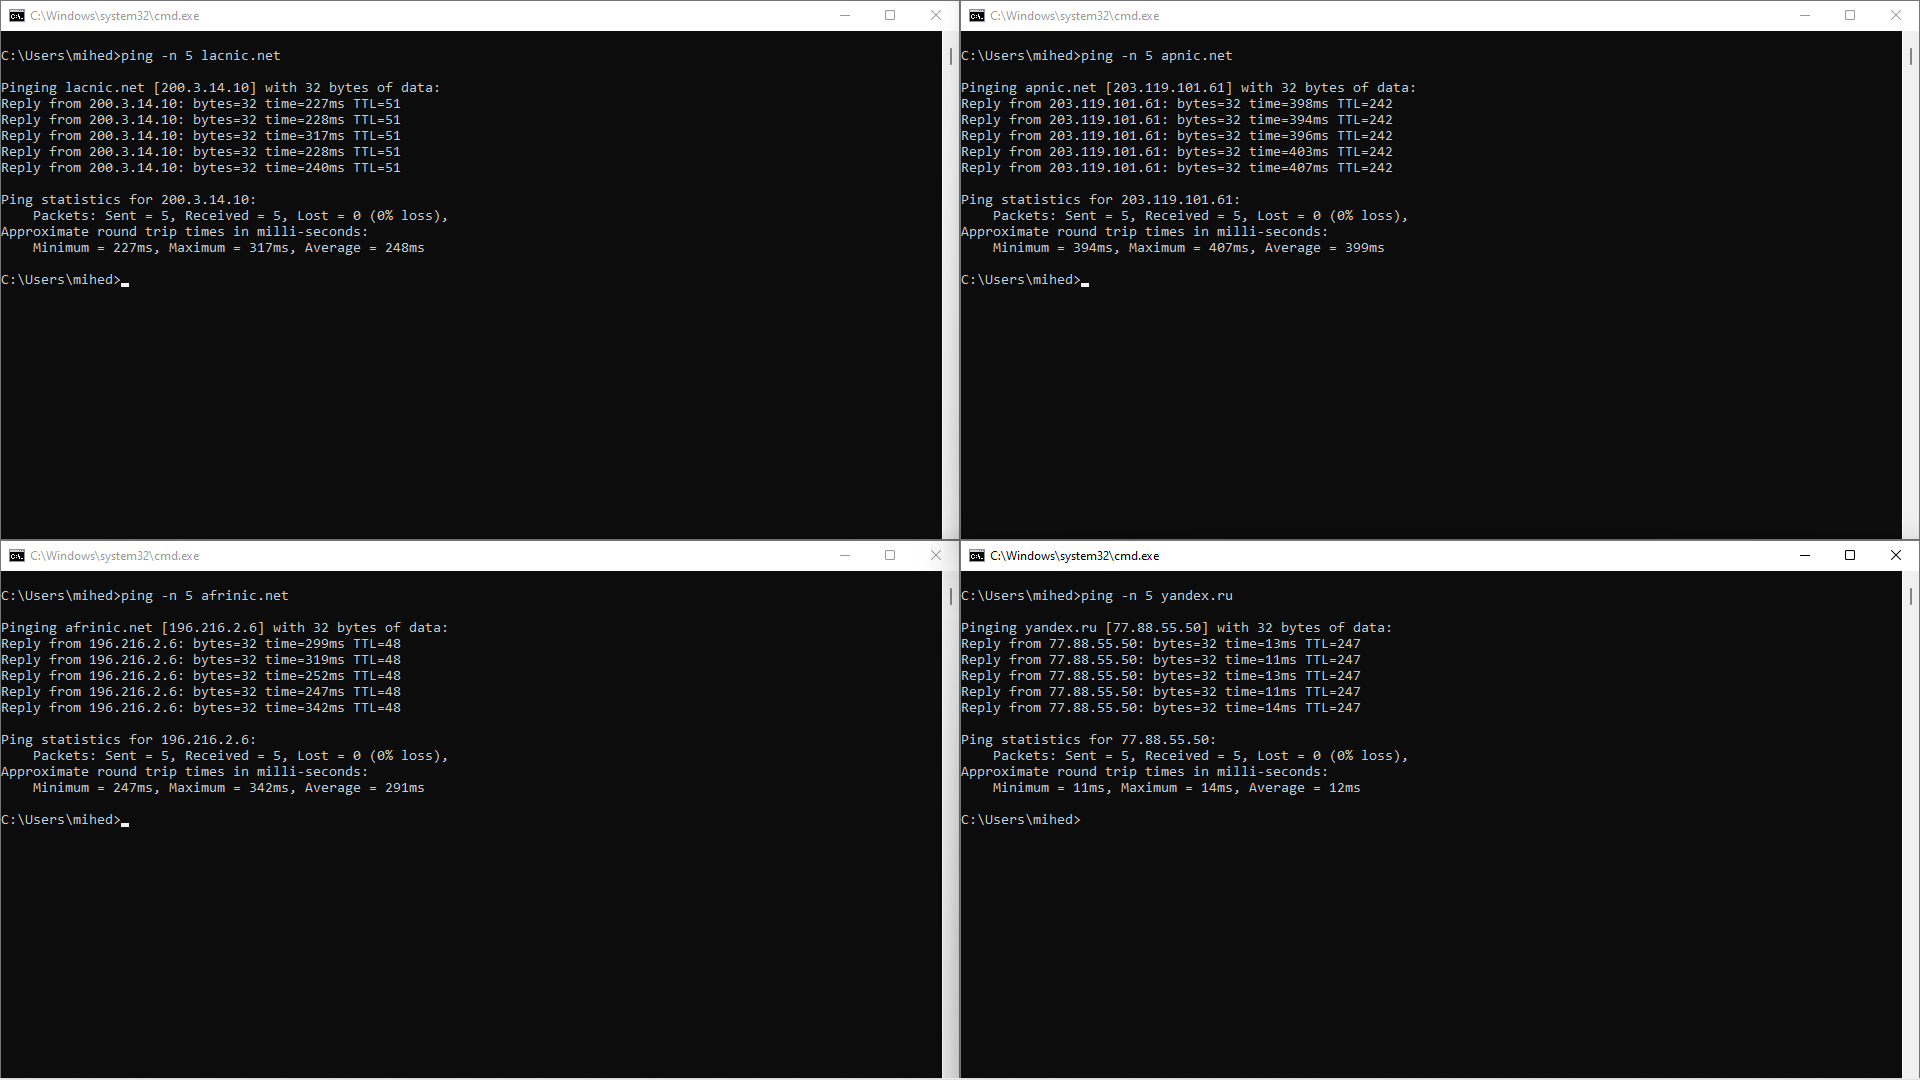
\includegraphics[width=0.85\textwidth]{05_0001}
    \caption{Пингуем необходимые ресурсы}
    \label{img:0001}
  \end{figure}

  Полученные данные можно сопоставить с удаленностью ресурсов от удаленной машины, для 
  этого составим таблицу:
  \begin{table}[H]
    \centering
    \begin{tabular}{| c | c | c | c | c | c |}
      \hline
      \multirow{2}{*}{Сервис} & \multirow{2}{*}{Местоположение} & \multicolumn{3}{| c |}{Время ответа} & \multirow{2}{*}{TTL} \\
      \cline{3-5}
      & & Минимальное & Среднее & Максимальное & \\
      \hline
      \href{yandex.ru}{yandex.ru} & Россия & 11ms & 12ms & 14ms & 247 \\
      \hline
      \href{lacnic.net}{lacnic.net} & Южная Америка & 227ms & 248ms & 317ms & 51 \\
      \hline
      \href{afrinic.net}{afrinic.net} & Африка & 247ms & 291ms & 342ms & 48 \\
      \hline
      \href{apnic.net}{apnic.net} & Австралия & 394ms & 399ms & 407ms & 242 \\
      \hline
    \end{tabular}
    \caption{Время ответа для различных ресурсов}
  \end{table}

  Как видно из полученных данных - быстрее всего ответ приходит от сервиса, расположенного в России.
  Это происходит потому, что сервера географически находятся ближе и пакетам нужно физически преодолеть меньшее 
  расстояние. Пакеты, отправленные в Южную Америку шли значительно дольше - им потребовалось пересечь
  Атлантический океан и вернуться обратно, что и заняло большую часть времени.
  Ответ из Африки был также получен за значительное время, возможно, это обусловлено качеством используемого
  там сетевого оборудования. Дольше всего пакеты шли до Австралии.

  Проанализируем промежуточные точки маршрутизации, для этого воспользуемя утилитой \textit{tracert}
  для анализа тех же сервисов (рис. \ref{img:0002} на стр. \pageref{img:0002}):
  \begin{figure}[H]
    \centering
    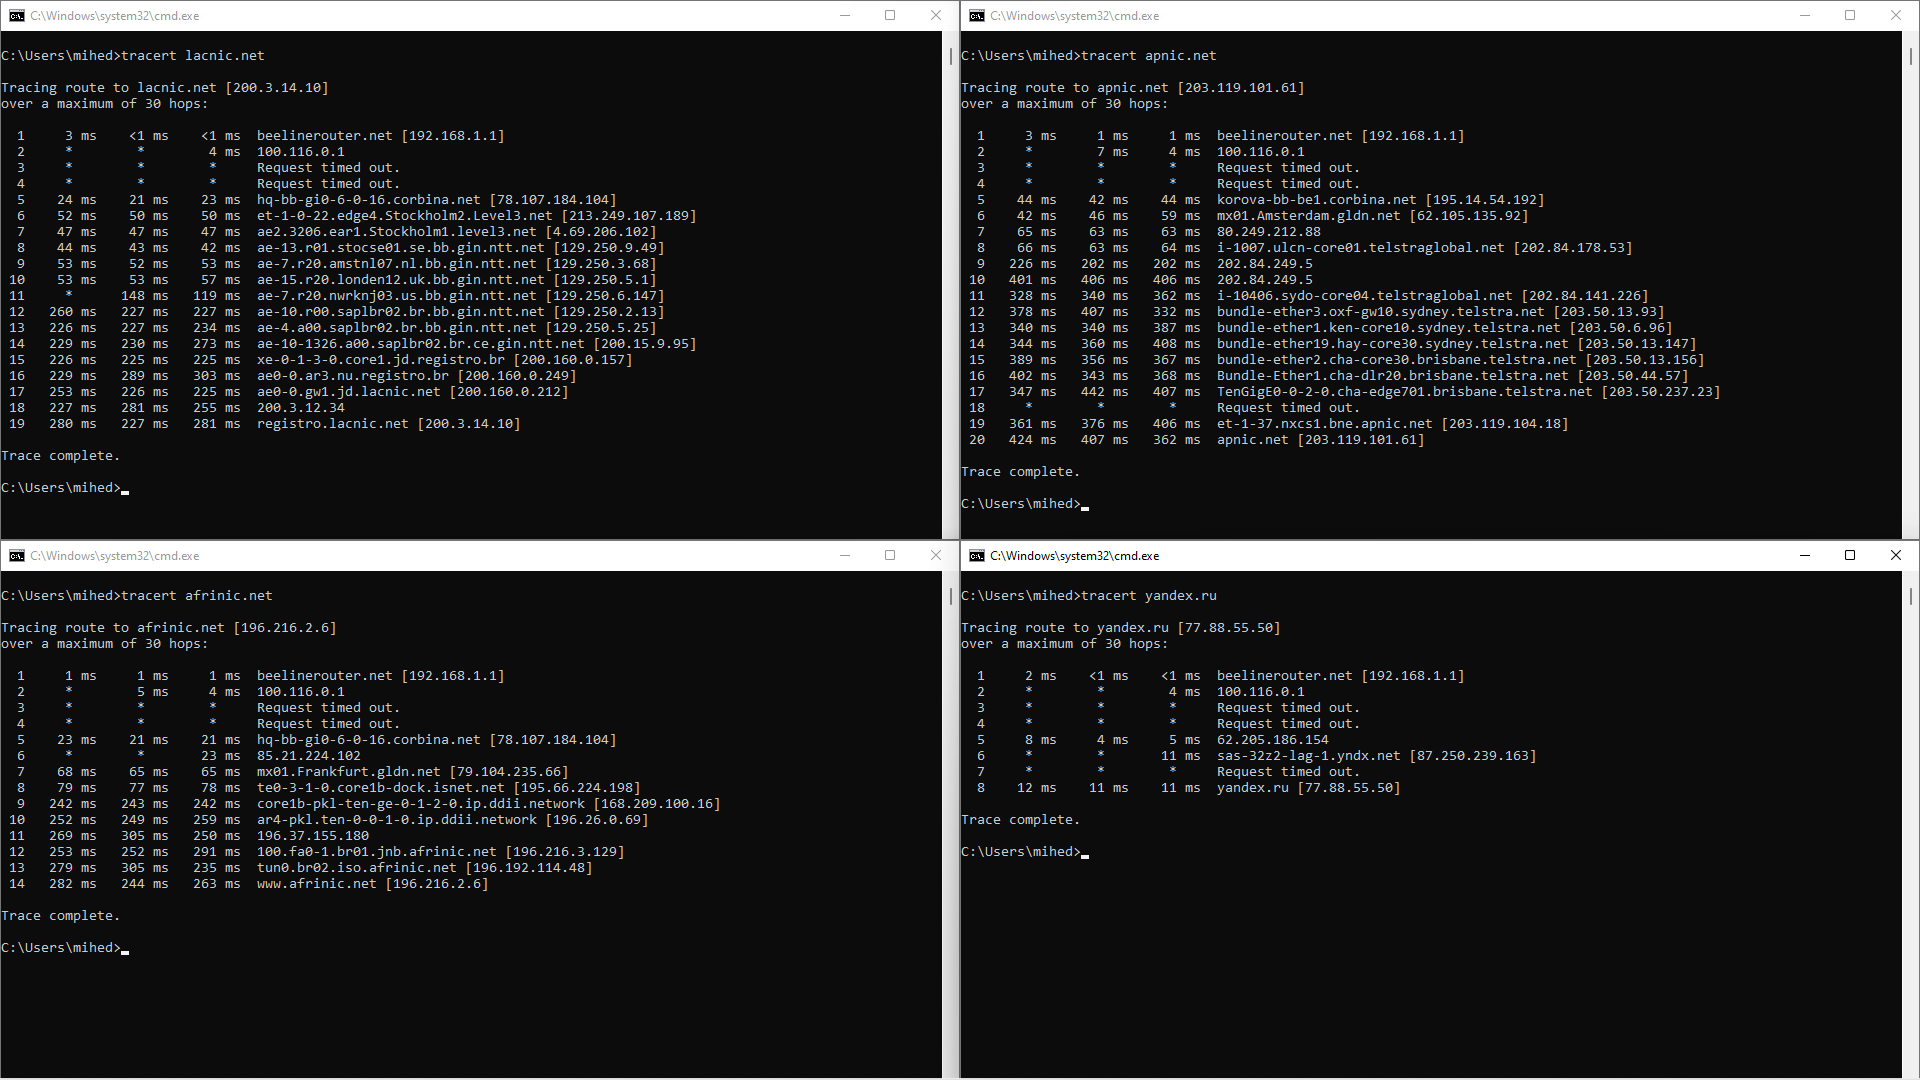
\includegraphics[width=0.85\textwidth]{05_0002}
    \caption{Анализ маршрута отправленных пакетов}
    \label{img:0002}
  \end{figure}

  Видно, что меньше всего прыжков (всего 8 штур) потребовалось для того, чтобы достичь \href{yandex.ru}{yandex.ru} что и
  логично, ведь сервера данного ресурса расположены ближе всего. Наибольшее же количество прыжков (целых 20)
  потребовалось, чтобы дойти до \href{apnic.net}{apnic.net} (Австралия), что объясняет долгое время получения
  ответа от данного сервера.

  \subsection{Анализ ресурса \href{cisco.com}{cisco.com}}

  Для начала проверим доступность ресурса при помощи \textit{ping} (рис. \ref{img:0003} на стр. \pageref{img:0003}):
  \begin{figure}[H]
    \centering
    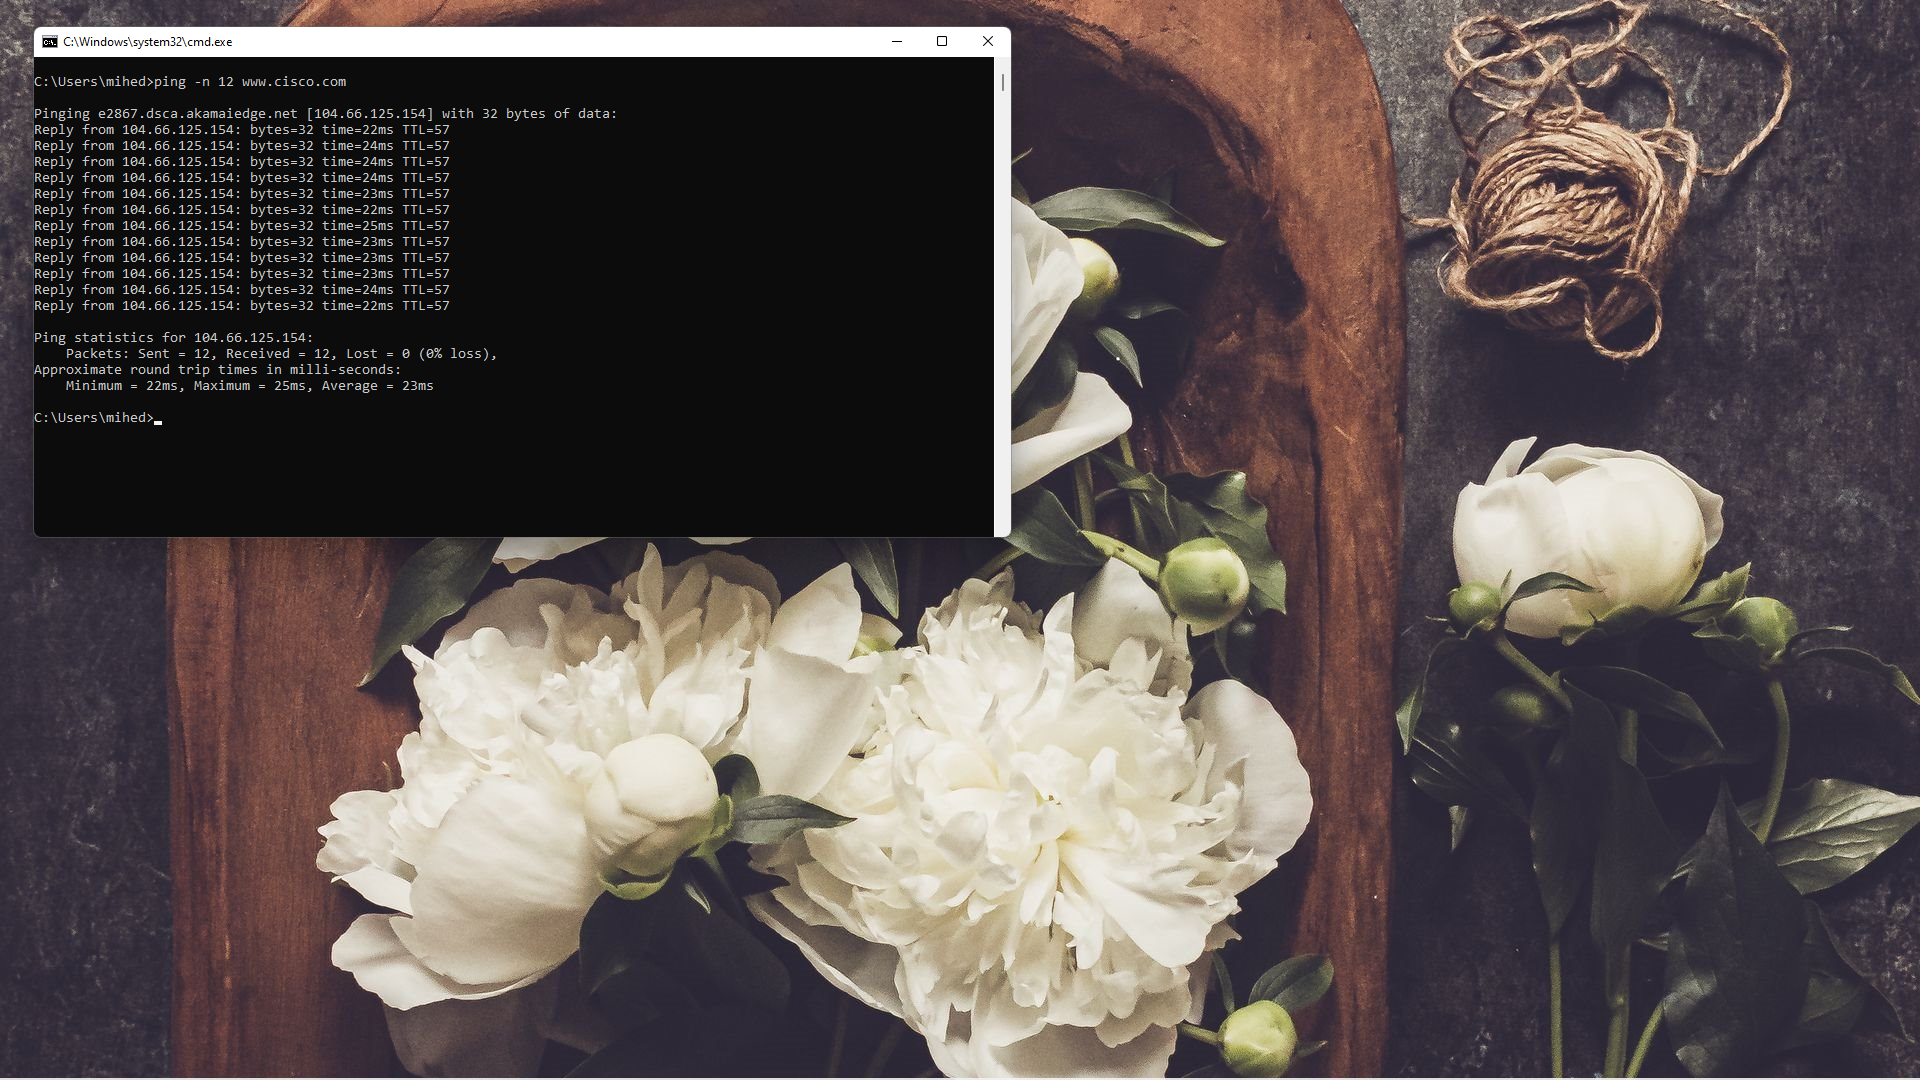
\includegraphics[width=0.85\textwidth]{05_0003}
    \caption{Пинг до cisco.com}
    \label{img:0003}
  \end{figure}

  Теперь изучим путь пакетов от рабочей машины до ресурса. Сдлеаем это 3-мя возможными способами:
  с помощью утилиты \textit{tracert}, с помощью специализированного ПО \textit{OpenVisualTraceroute}
  и с помощью Интернет-ресурса \href{https://2whois.ru/?t=traceroute}{2whois.ru}.

  \begin{figure}[H]
    \centering
    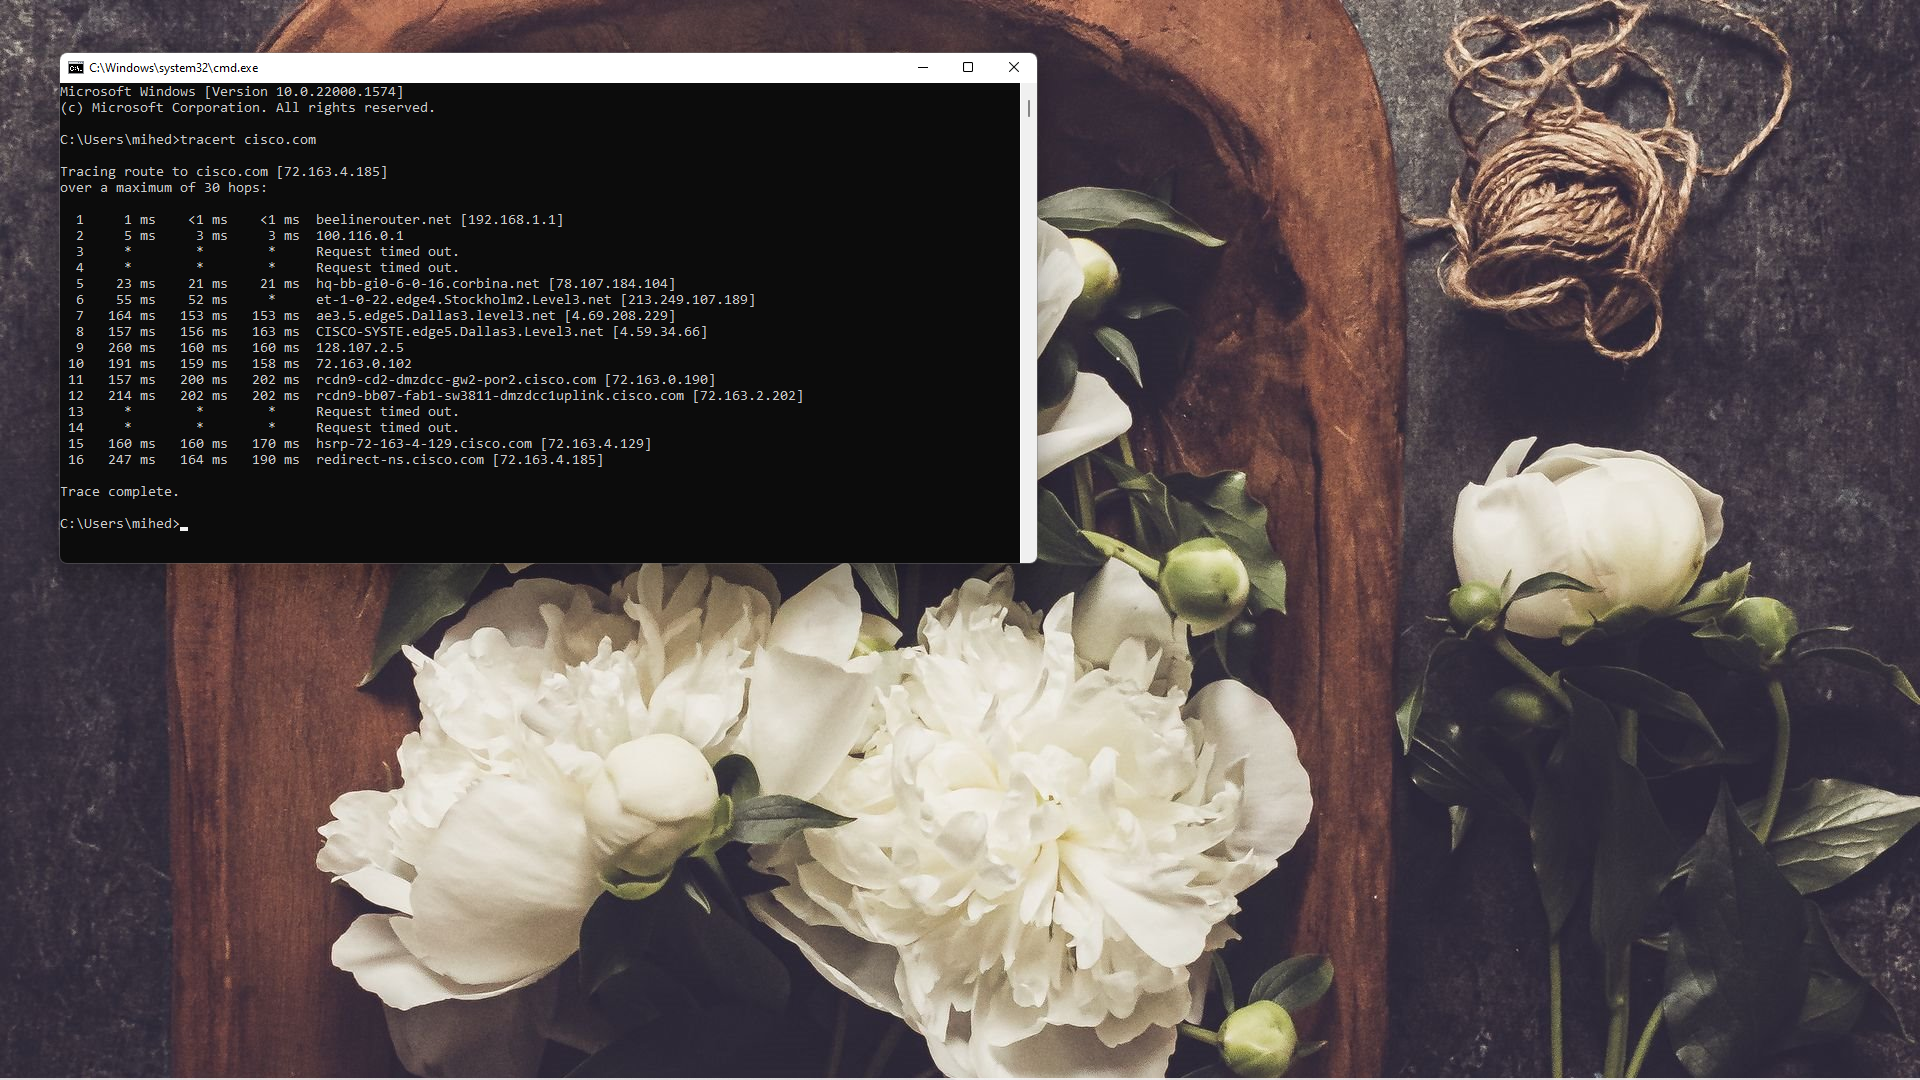
\includegraphics[width=0.85\textwidth]{05_0004}
    \caption{Анализ при помощи \textit{tracert}}
    \label{img:0004}
  \end{figure}

  \begin{figure}[H]
    \centering
    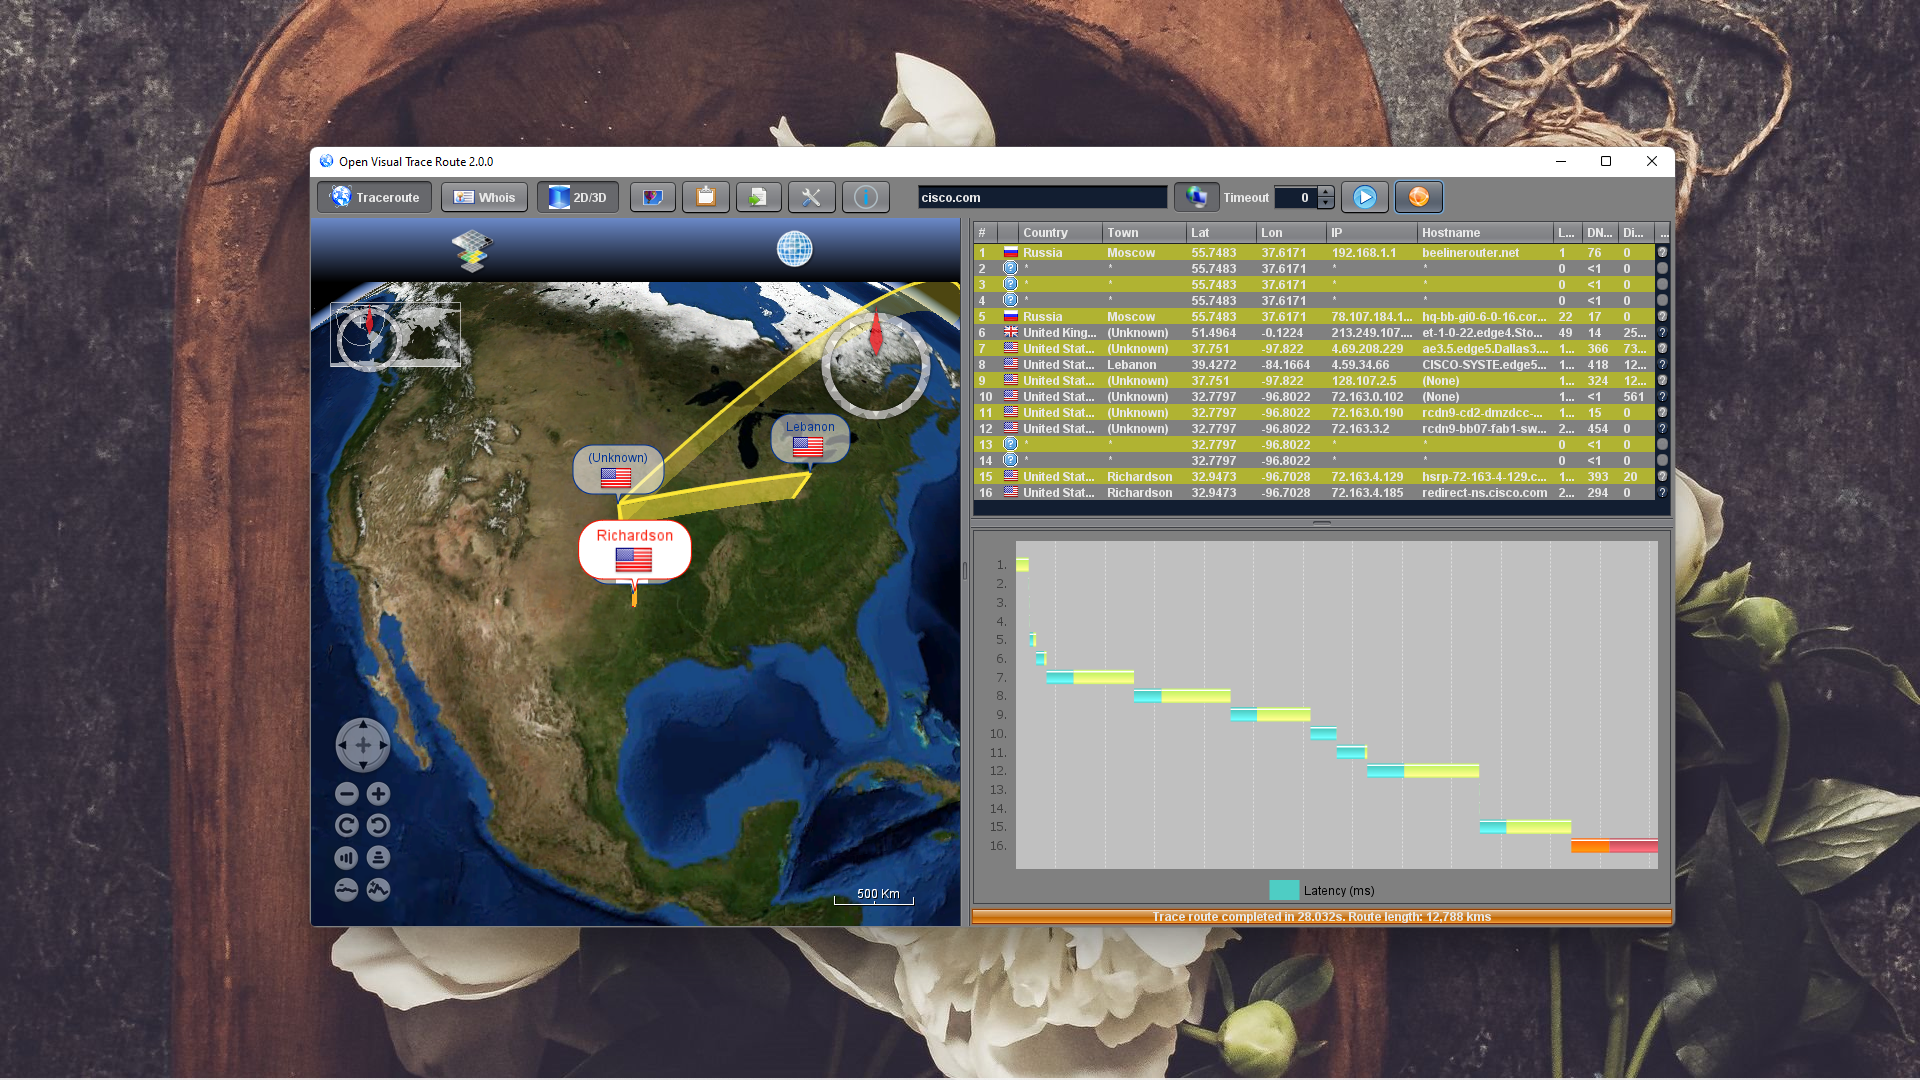
\includegraphics[width=0.85\textwidth]{05_0005}
    \caption{Анализ при помощи \textit{OpenVisualTraceroute}}
    \label{img:0005}
  \end{figure}
  
  \begin{figure}[H]
    \centering
    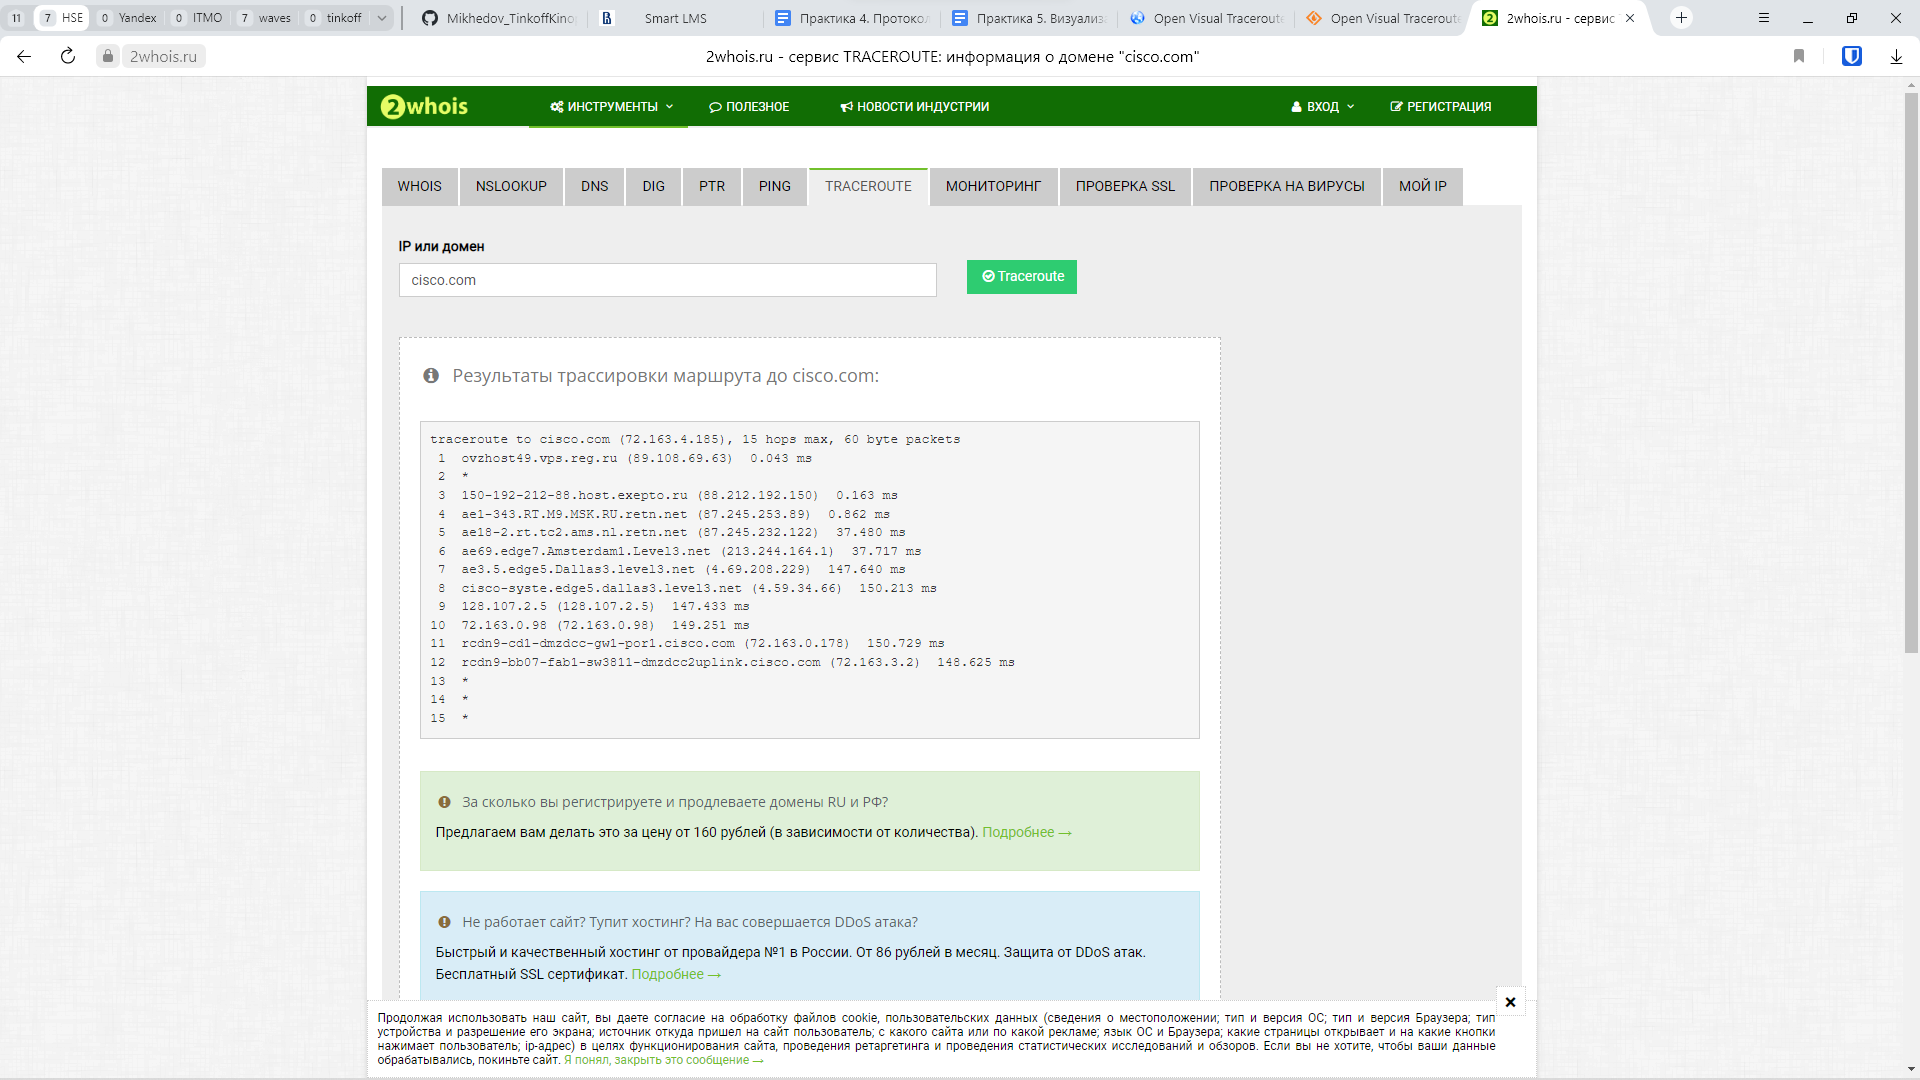
\includegraphics[width=0.85\textwidth]{05_0006}
    \caption{Анализ при помощи web-ресурса}
    \label{img:0006}
  \end{figure}

  Во-первых, необходимо отметить, что все отправленные пакеты в конечном итоге пришли на один
  и тот же \textit{IPv4}-адрес: 72.163.4.185. Во-вторых, все использованные инструменты выдали 
  практически один и тот же ответ: отличился только web-ресурс, он не учел один единственный адрес моего маршрутизатора,
  с помощью которого был получен доступ в сеть. Но это и правильно, так как на web-ресурс запрос на анализ пришел уже
  с маршрутизатора, а не напрямую с рабочей машины.

  В остальном же, результаты полученные при помощи утилит, запущенных локально, полностью совпадают,
  а вот web-ресурс видимо  изучал путь не от моей машины, а от того компьютера, на котором запущен сам.

  \newpage
  \section{Вывод}

  В ходе данной лабораторной работы я научился проверять доступность web-ресурсов при помощи утилиты \textit{ping},
  а также анализировать путь пакета от устройства к устройству с помощью разлитчного програмного обеспечения.
  \end{document}
